\documentclass[12pt]{article}
\usepackage{amsmath}
\usepackage{amsfonts}
\usepackage{parskip}
\usepackage{amsthm}
\usepackage{thmtools}
\usepackage[headheight=15pt]{geometry}
\geometry{a4paper, left=20mm, right=20mm, top=30mm, bottom=30mm}
\usepackage{graphicx}
\usepackage{bm} % for bold font in math mode - command is \bm{text}
\usepackage{enumitem}
\usepackage{fancyhdr}
\usepackage{amssymb} % for stacked arrows and other shit
\pagestyle{fancy}
\usepackage{changepage}
\usepackage{mathcomp}
\usepackage{tcolorbox}

\declaretheoremstyle[headfont=\normalfont]{normal}
\declaretheorem[style=normal]{Theorem}
\declaretheorem[style=normal]{Proposition}
\declaretheorem[style=normal]{Lemma}
\newcounter{ProofCounter}
\newcounter{ClaimCounter}[ProofCounter]
\newcounter{SubClaimCounter}[ClaimCounter]
\newenvironment{Proof}{\stepcounter{ProofCounter}\textsc{Proof.}}{\hfill$\square$}
\newenvironment{claim}[1]{\vspace{1mm}\stepcounter{ClaimCounter}\par\noindent\underline{\bf Claim \theClaimCounter:}\space#1}{}
\newenvironment{claimproof}[1]{\par\noindent\underline{Proof of claim \theClaimCounter:}\space#1}{\hfill $\blacksquare$ Claim \theClaimCounter}
\newenvironment{subclaim}[1]{\stepcounter{SubClaimCounter}\par\noindent\emph{Subclaim \theClaimCounter.\theSubClaimCounter:}\space#1}{}
% \newenvironment{subclaimproof}[1]{\begin{adjustwidth}{2em}{0pt}\par\noindent\emph{Proof of subclaim \theClaimCounter.\theSubClaimCounter:}\space#1}{\hfill
% $\blacksquare$ \emph{Subclaim \theClaimCounter.\theSubClaimCounter}\vspace{5mm}\end{adjustwidth}}
\newenvironment{subclaimproof}[1]{\par\noindent\emph{Proof of subclaim \theClaimCounter.\theSubClaimCounter:}\space#1}{\hfill
$\Diamond$ \emph{Subclaim \theClaimCounter.\theSubClaimCounter}}

\allowdisplaybreaks{}

% chktex-file 3

\title{STAT 520: HW 2}
\author{Evan P. Walsh}
\makeatletter
\makeatother
\lhead{Evan P. Walsh}
\chead{STAT 520: HW 2}
\rhead{\thepage}
\cfoot{}

\begin{document}
\maketitle



\subsection*{1}
The natural choice for a two sample model would be a model with different $\alpha$ and $\beta$ parameters for each group, where all observations are
treated as independent. That is, we assume 
$Y_{1,1}, \dots, Y_{1,n_1}$ iid $\sim$ Gamma$(\alpha_1, \beta_1)$ and $Y_{2,1}, \dots, Y_{2,n_2}$ iid $\sim$ Gamma$(\alpha_2, \beta_2)$.
Of course, without knowing the context of the problem it is impossible to say whether or not the assumption of independence can be justified, much
less the assumption that these random variables follow a Gamma distribution. We bravely proceed anyway.

Let $\bm{y}_1 := (y_{1,1}, \dots, y_{1,n_1})$ and $\bm{y}_2 := (y_{2,1}, \dots, y_{2,n_2})$. For group 1, the log likelihood function is given by
\begin{align*}
  \ell(\alpha_1,\beta_1|\bm{y}_1) & = \log\left\{ \prod_{i=1}^{n_1} \frac{\beta_{1}^{\alpha_1}}{\Gamma(\alpha_1)}y_{1,i}^{\alpha_1 - 1} \exp(-\beta_1
  y_{1,i}) \right\} \\
  & = n_1 \alpha_1 \log(\beta_1) - n_1 \log[\Gamma(\alpha_1)] - \beta_1 \sum_{i=1}^{n_1}y_{1,i} + (\alpha_1 - 1)\sum_{i=1}^{n_1}\log(y_{1,i}).
\end{align*}

In order to maximize this function using the Newton-Raphson method, we will also need to compute
\begin{align*}
  & \frac{\partial}{\partial \alpha_1}\ell(\alpha_1,\beta_1|\bm{y}_1) = n_1 \log(\beta_1) - \frac{n_1 \Gamma'(\alpha_1)}{\Gamma(\alpha_1)} +
  \sum_{i=1}^{n_1}\log(y_{1,i}) \\
  & \frac{\partial^2}{\partial \alpha_{1}^{2}}\ell(\alpha_1,\beta_1|\bm{y}_1) = -n_1\frac{\Gamma(\alpha_1)\Gamma''(\alpha_1) -
  [\Gamma'(\alpha_1)]^{2}}{[\Gamma(\alpha_1)]^{2}} \\
  & \frac{\partial}{\partial \alpha_1}\frac{\partial}{\partial \beta_1}\ell(\alpha_1,\beta_1|\bm{y}_1) = 
  \frac{\partial}{\partial \beta_1}\frac{\partial}{\partial \alpha_1}\ell(\alpha_1,\beta_1|\bm{y}_1) = \frac{n_1}{\beta_1} \\
  & \frac{\partial}{\partial \beta_1}\ell(\alpha_1,\beta_1|\bm{y}_1) = \frac{n_1\alpha_1}{\beta_1} - \sum_{i=1}^{n_1}y_i \\
  & \frac{\partial}{\partial \alpha_1}\ell(\alpha_1,\beta_1|\bm{y}_1) = -\frac{n_1 \alpha_1}{\beta_{1}^{2}}.
\end{align*}


\subsection*{2}

We used the Newton-Raphson method to find the maximum likelihood estimates for $\alpha$, and $\beta$ in the full model with two groups and the reduced
model with one group. 
In each case the method of moments estimators were used as starting values for the algorithm.
For Group 1 and Group 2, the log likelihood was maximized at $(\hat{\alpha}_1, \hat{\beta}_1) = (4.563441, 2.412541)$ and 
$(\hat{\alpha}_2, \hat{\beta}_1) = (1.043059, 0.540959)$, respectively, after 9 iterations for each. For the reduced model, the best estimates were found to be 
$(\hat{\alpha}, \hat{\beta}) = (1.6522803, 0.8651324)$ after 7 iterations. 

We also computed 95\% Wald theory confidence intervals using the result that the MLE's are asymptotically normal with a covariance matrix that can be
approximated with the observed Fisher Information matrix. The results are summarized in the table below.

\begin{table}[h]
  \begin{center}
    \begin{tabular}{|l|c|c|c|c|}
      \hline
      & $\hat{\alpha}$ & 95\% Wald CI for $\alpha$ & $\hat{\beta}$ & 95\% Wald CI for $\beta$ \\
      \hline 
      Group 1 & 4.5634 & (2.1205, 7.0064) & 2.4125 & (1.0473, 3.7778) \\
      \hline
      Group 2 & 1.0531 & (0.5320, 1.5541) & 0.5410 & (0.2043, 0.8776) \\
      \hline
      Reduced & 1.6523 & (1.0585, 2.2461) & 0.8651 & (0.5025, 1.2277) \\
      \hline
    \end{tabular}
  \end{center}
  \caption{MLE estimates and 95\% Wald theory confidence intervals.}
\end{table}



\subsection*{3}

To test whether the groups should be considered significantly different, we compute the test statistic
\[
  T := -2\left\{ \ell_{\text{R}} - \ell_{\text{F}} \right\} = -2\left\{ -79.071 - (-30.503 - 41.400) \right\} = 14.335,
\]
where $\ell_{\text{R}}$ is the log likelihood evaluated at the estimates of the parameters for the reduced model and $\ell_{\text{F}}$ is the log likelihood evaluated
at the estimates of the parameters for the full model. Given that the Gamma distribution is a regular exponential family, test statistics in the form
of $T$ will have the limiting distribution of a $\chi_{2}^{2}$ random variable. The 2 degrees of freedom come from the difference in dimensionality of
the full parameter space versus the reduced parameter space. The p-value found by comparing the test statistic its limiting distribution is 0.00077,
far below the threshold of 0.10. Hence there is significant evidence that the full model with separate parameters for each group is a better fit than
the reduced model.


\subsection*{4}

Figure 1 shows a plot of the estimated distribution functions for both groups.

\begin{figure}[!h]
  \caption{Estimated density functions for both groups}
  \centering
  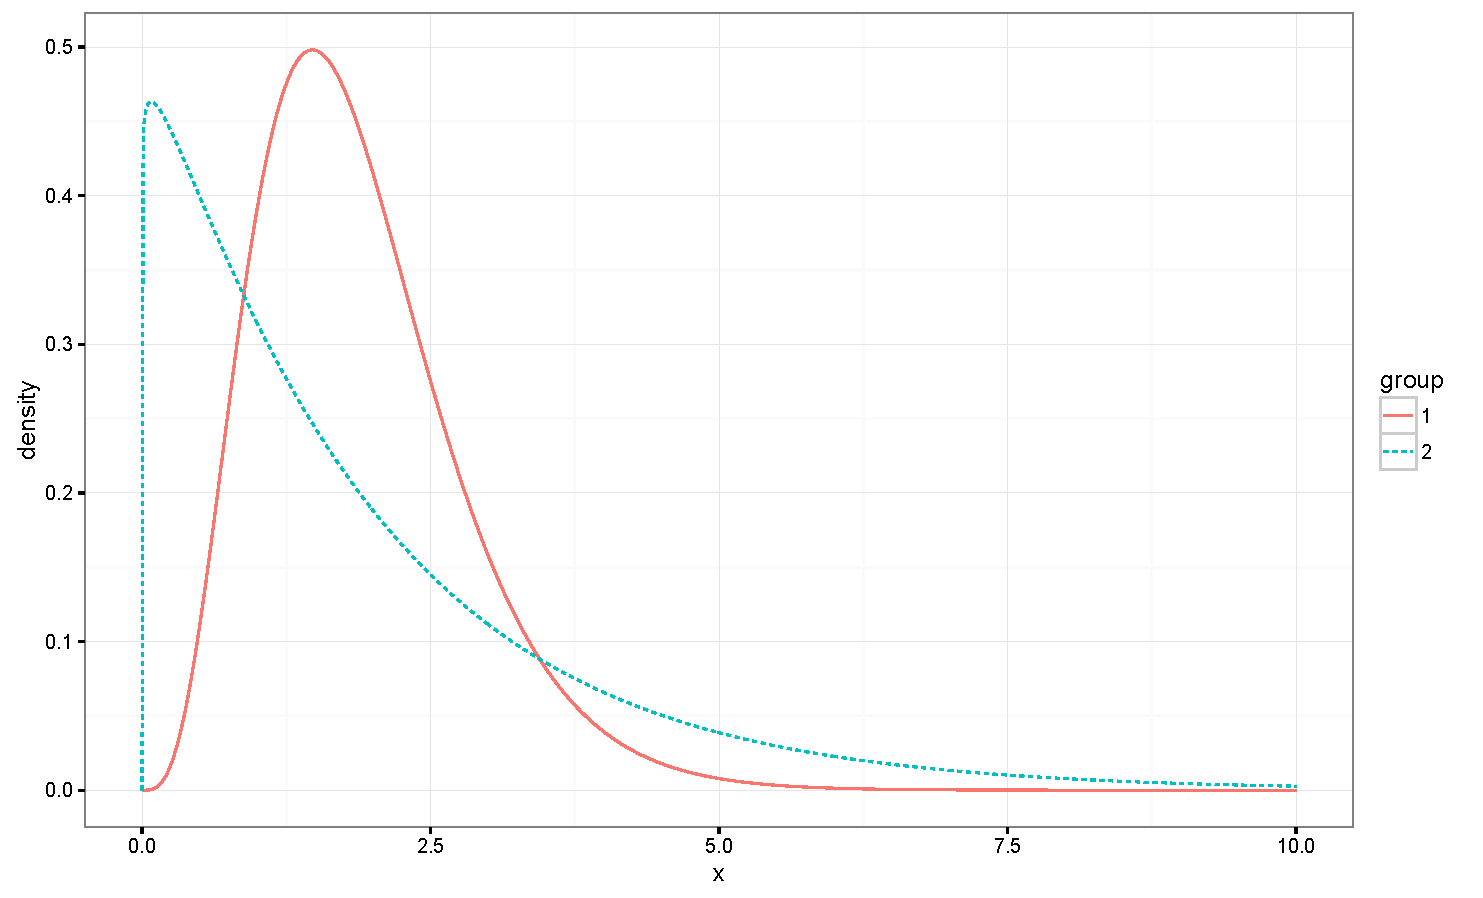
\includegraphics[width=0.9\textwidth]{./figures/hw02_group.pdf}
\end{figure}


\subsection*{5}

We now test whether the groups should be considered significantly different using a two-sample t-test. In particular, this means we are testing for a
difference in group means. Note that the sample variance of Group 1 is 0.6948 while the sample variance of Group 2 is 3.5210, which seem very
different. Hence we conduct the t-test assuming that the variances of both groups differ. The null and alternative hypothesis are 
\[
  \text{H}_{0}: \mu_1 = \mu_2 \qquad \text{ and } \qquad \text{H}_1: \mu_1 \neq \mu_2,
\]
where $\mu_1 = \alpha_1 / \beta_1$ is the expected value for Group 1 and $\mu_2 = \alpha_2 / \beta_2$ is the expected value for Group 2.
The test statistic is 
\[
  t = \frac{\bar{y}_1 - \bar{y}_2}{\sqrt{ \frac{s_{1}^{2}}{n_{1}} + \frac{s_{2}^{2}}{n_{2}}}} = -0.089151.
\]
The resulting two-sided p-value obtained by comparing $t$ to a t-distribution with 33.112 degrees of freedom is 0.9295. 
Thus we fail to reject the null hypothesis. So there is no evidence that the mean for Group 1 is
different from the mean for Group 2.


\subsection*{6}

Using the invariance of maximum likelihood estimators we obtain the following point estimates for the group means:
\[
  \hat{\mu}_1 := \frac{\hat{\alpha}_1}{\hat{\beta}_1} = 1.8915 \qquad \hat{\mu}_2 := \frac{\hat{\alpha}_2}{\hat{\beta}_2} = 1.9282. 
\]
Using the multivariate delta method, the variance of $\hat{\mu}_j$, $j = 1,2$, can be estimated as 
\[
  \widehat{\text{var}}(\hat{\mu}_j) = D(\alpha, \beta)^{T} I^{-1}(\alpha,\beta) D(\alpha, \beta) \bigg|_{\alpha = \hat{\alpha}_j, \beta = \hat{\beta}_j},
\]
where $D(\alpha, \beta) := \left[ \beta^{-1}, -\alpha \beta^{-2} \right]$ and $I^{-1}(\alpha, \beta)$ is the invserse of the Fisher Information matrix.
A 95\% confidence interval for the difference in group means is therefore given by 
\[
  (\hat{\mu}_1 - \hat{\mu}_2) \pm 1.96 * \sqrt{ \widehat{\text{var}}(\hat{\mu}_1) + \widehat{\text{var}}(\hat{\mu}_2) } = (-0.8541, 0.7808).
\]
Since 0 is within the interval, there is not sufficient evidence for a difference in group means.


\subsection*{7}

In Part 3 we found that there was significant evidence that the groups came from different Gamma distributions based on a likelihood ratio test.
However, the 2-sample t-test in Part 5 revealed that there was not a significant difference between the means of both groups. This result was corroborated by
another test in Part 6 for difference in group means using the invariance property of MLEs and the multivariate delta method.



\end{document}
